\chapter{Data: Representation}

When inputting data into a model, we need to consider the structure of the data.
First we must consider the \textit{modality}:
\begin{itemize}
    \item \textbf{Image:} Tensor of height $\times$ width $\times$ colour.
    \item \textbf{Video:} Tensor of height $\times$ width $\times$ colour $\times$ time.
    \item \textbf{Text:} List of \textsc{string}. 
    \item \textbf{Time Series:} Tensor of value $\times$ time. 
    \item The list goes on.
\end{itemize}
Each of these must be transformed into something a model can act upon.

\section{Embedding}
\label{sec:representation-embeddings-as-operational-geometry}
First up, many complex data inputs (text, time series, images) exist in a space that humans can explore (through our eyes, ears, time) but that models cannot.
Embedding is a method of transforming these into a vector space, such that each datapoint exists somewhere in the vector space.
We use an \textit{encoder} for this transformation.
We choose a number of dimensions for this vector space based on computational cost and downstream usefulness.

In theory, similar starting datapoints should be close together in the embedding space - although this is not always true, due to non-linear encodings.

\begin{figure}[htbp]
    \centering
    \begin{tikzpicture}[node distance=9mm and 12mm]
    \node[flow] (obj) {Text / image\\user / item};
    \node[flow,right=of obj] (enc) {Encoder};
    \node[yesbox,right=of enc] (vec) {Embedding\\$z\in\R^{N_{\text{embedding dims}}}$};
    \node[flow,right=of vec] (sim) {Similarity\\dot / cosine};
    \node[yesbox,right=of sim] (near) {Nearest\\neighbours};
    \draw[arr] (obj)--(enc);
    \draw[arr] (enc)--(vec);
    \draw[arr] (vec)--(sim);
    \draw[arr] (sim)--(near);
    \end{tikzpicture}
    \caption{A nearest neighbours embedding use-case.}
\end{figure}

\begin{calloutdegreeofexperiment}
Vary encoder objective, embedding dimension, normalisation, similarity function, compression/quantisation and whether one representation must support several retrieval budgets.
\end{calloutdegreeofexperiment}

\paragraph{L2-Normalised Embeddings}
If embeddings are L2-normalised, then the cosine distance metric becomes a simple dot product.
Computing a raw dot product is much faster than computing cosine similarity because it completely skips the square root and division operations required to find vector magnitudes.
Vector databases (like Milvus, Pinecone, or Qdrant) can use hardware-accelerated dot product instructions (MADD / AVX) to search through L2-normalised embeddings at scale, giving you the directional benefits of cosine similarity with the raw speed of a dot product.
A common design question is therefore whether embedding norm should carry task information.


\paragraph{Information Ordered Dimensions}
\textbf{Matryoshka}-style representations ensure that the most important information is packed into the earlier dimensions of a vector, moving part of the quality--cost choice from retraining time to serving time.
\[
    [z_1,\ldots,z_{64}]
    \subset
    [z_1,\ldots,z_{128}]
    \subset
    [z_1,\ldots,z_{N_{\text{embedding dims}}}].
\]
Conceptually, this is \textit{kind of} like making succesive vector spaces out of residuals - however this is not what actually happens.

\paragraph{Quantisation}
Quantising vector element values to fewer bits offers large memory savings.
It is safe to do when the distance metric results remains identical.
This connects directly to model quantisation in \cref{sec:inference-quantisation} and vector search in \cref{sec:llms-rag,sec:ranking-retrieval}.

\section{Tokenisers}
Some data structures, like text and some time-series, are sequences of categories in a very high dimensional space.
For example, there are \textit{about} 26 thousand words in English, and a sentence can be thought of as a path between these words. 
To represent these to models we order the categories and assign them an integer ID number per category.
Those IDs index an embedding matrix:
\[
    E_{\text{token embedding}}
    \in
    \mathbb{R}^{N_{\text{vocabulary}}\times N_{\text{representation dims}}}.
\]
If token ID $791$ occurs, row $791$ is retrieved and its embedding vector available.
The tokeniser itself is normally trained before the language model, so the model inherits those boundaries rather than learning them jointly with its representations.
So the full pipeline is:
\begin{figure}[htbp]
    \centering
    \begin{tikzpicture}[node distance=8mm and 8mm]
    \node[flow] (chars) {Characters};
    \node[flow,right=of chars] (tok) {Tokeniser};
    \node[yesbox,right=of tok] (ids) {Discrete\\token IDs};
    \node[flow,right=of ids] (emb) {Embedding\\lookup};
    \node[yesbox,right=of emb] (vec) {Continuous\\vectors};
    \node[flow,right=of vec] (net) {Neural\\network};
    \draw[arr] (chars)--(tok);
    \draw[arr] (tok)--(ids);
    \draw[arr] (ids)--(emb);
    \draw[arr] (emb)--(vec);
    \draw[arr] (vec)--(net);
    \end{tikzpicture}
    \label{fig:modern-tokenisation-flow}
\end{figure}
For example:
\begin{align}
    &\texttt{``The unbelievable result''}
    \rightarrow
    [\texttt{The},\ \texttt{ unbeliev},\ \texttt{able},\ \texttt{ result}]
    \rightarrow
    \\
    &\rightarrow
    [791,42291,481,1121]
    \rightarrow
    [\mathbf{e}_{791},\mathbf{e}_{42291},\mathbf{e}_{481},\mathbf{e}_{1121}]
    \rightarrow
    \begin{gathered}
    \begin{bmatrix}
        0.12 & -0.43 & 0.87 & 0.21\\
        -0.56 & 0.31 & 0.14 & -0.72\\
        0.93 & -0.18 & 0.45 & 0.06\\
        -0.24 & 0.67 & -0.39 & 0.81
    \end{bmatrix}\\[-1pt]
    \begin{array}{cccc}
        \underbrace{\hphantom{0.12}}_{\mathbf{e}_{791}} &
        \underbrace{\hphantom{-0.43}}_{\mathbf{e}_{42291}} &
        \underbrace{\hphantom{0.87}}_{\mathbf{e}_{481}} &
        \underbrace{\hphantom{0.21}}_{\mathbf{e}_{1121}}
    \end{array}
    \end{gathered}
\end{align}

\begin{tikzpicture}[node distance=7mm and 7mm]
    % Tokenisation pipeline
    \node[flow] (raw) {Raw text};
    \node[flow,right=of raw] (norm) {Normalise\\text};
    \node[flow,right=of norm] (pre) {Impose coarse\\pre-token boundaries};
    \node[flow,right=of pre] (seg) {Segment pieces\\using learned vocabulary};
    \node[flow,right=of seg] (map) {Map tokens\\to integer IDs};
    \node[yesbox,right=of map] (ids) {Token\\IDs};
    
    \draw[arr] (raw) -- (norm);
    \draw[arr] (norm) -- (pre);
    \draw[arr] (pre) -- (seg);
    \draw[arr] (seg) -- (map);
    \draw[arr] (map) -- (ids);
    
    % Tokeniser training
    \node[yesbox,below=12mm of seg] (vocab)
        {Learned vocabulary +\\segmentation rules};
    \node[flow,left=of vocab] (train)
        {Tokeniser\\training corpus};
    
    \draw[arr] (train) -- (vocab);
    \draw[arr] (vocab) -- (seg);
\end{tikzpicture}

\paragraph{Level Of Tokeniser}
There are many ways to skin a word, each with different biases. 
For example:
\begin{itemize}
    \item \textit{Why not use words?}
    Because it is not the most efficient decomposition of meaning. 
    It woudl complicate pre/suf-fixes, plurals and other semantic means we use grammar to encode. 
    \item  \textit{Why not use letters?}
    Because the number of possible permutations is enormous.
\end{itemize}

Imagine the token count differences between:
\begin{align}
    & \texttt{[transformational]} \rightarrow \texttt{[transform, ational]} \\
    & \texttt{[transformational]} \rightarrow \texttt{[trans, form, ation, al]} \\
    & \texttt{[transformational]} \rightarrow \texttt{[t, r, a, n, s, f, o, r, m, a, t, i, n, o, a, l]}
\end{align}

The trade-off is vocabulary capacity against sequence length:
\[
    \underbrace{N_{\text{vocabulary}}N_{\text{representation dims}}}_{\text{token embedding parameters}}
    \quad\leftrightarrow\quad
    \underbrace{N_{\text{tokens}}}_{\text{sequence length}}
    \quad\Rightarrow\quad
    \underbrace{N_{\text{tokens}}^2}_{\text{dense attention interactions}}.
\]
A larger vocabulary can compress common strings into fewer model steps (remember that transformers need to \textit{do an inference pass} for each token in a sequence), but spends more parameters on the discrete interface and creates more specialised units.
Smaller units improve coverage and sharing, but lengthen the sequence and consume more context and attention work.

\begin{calloutdegreeofexperiment}
Vary vocabulary size, BPE versus Unigram-style segmentation, byte fallback, multilingual vocabulary allocation, text normalisation and special-token design.
\end{calloutdegreeofexperiment}


\paragraph{Byte-Pair Encoding}
Byte-Pair Encoding (BPE) starts from small units and repeatedly merges the most frequent adjacent pair in the tokenizer-training corpus.
Heuristically,
\[
    [\texttt{l},\texttt{o},\texttt{w}]
    \rightarrow
    [\texttt{lo},\texttt{w}]
    \rightarrow
    [\texttt{low}].
\]
The learned merge ordering is then used to segment new text.
The key assumption is that frequently co-occuring characters should be represented as one object.
This produces useful compression, but frequent strings need not align with human linguistic units.

\paragraph{Unigram}
Unigram removes pieces instead. 
It starts with a large candidate vocabulary, fits a probabilistic segmentation model, then repeatedly removes pieces whose deletion damages the model least.
The useful differentiator is therefore:
\[
    \underbrace{\text{BPE}}_{\text{start small and merge}}
    \qquad\text{vs}\qquad
    \underbrace{\text{Unigram}}_{\text{start large and prune}}.
\]
\paragraph{SentencePiece} SentencePiece is tooling that can implement Unigram or BPE-style tokenisation.

\paragraph{WordPiece} WordPiece is another subword family, as used in BERT, but the heuristic is also the vocabulary-learning objective and the search procedure are design choices rather than immutable parts of ``tokenisation''.
It solves out of vocabulary issues by decomposing unknown words to continuation tokens.


\paragraph{Computational Cost}
Multilingual tokenisers learn a finite vocabulary from a mixture of languages, so high-resource text can receive more reusable pieces while underrepresented languages are split more finely.
The same effect appears for code, mathematical notation, unusual Unicode and numbers: inefficient segmentation means more model steps for the same underlying content.

\paragraph{Byte Fallback}
Byte fallback avoids a hard unknown-token failure by representing unsupported text through bytes, but can make rare strings much longer.

\begin{calloutpractical}
Do not compare per-token perplexity across different tokenisers as though a token were a fixed unit, because the prediction unit itself changed.
\end{calloutpractical}


\subsection{Tokens To Know}

Tokenisers use several conventions to represent subwords, word boundaries, unknown inputs, structural delimiters, and model-specific control information. 
Some are visible markers used when displaying a tokeniser's vocabulary. 
Exact token spellings and availability depend on the model and tokeniser version.
Be aware of these.

\subsubsection{The Classics}

\begin{itemize}
    \item \tok{[UNK]}: Unknown token used when an input cannot be represented by the vocabulary. Common in BERT/WordPiece.
    \item \tok{##}: WordPiece continuation prefix, used by BERT. For example, [\tok{play}, \tok{##ing}] represents ``playing''. The prefix indicates that a piece continues an existing word; it is not a standalone special token.
    \item \tok{</w>}: End-of-word marker used in early BPE implementations, including the original subword-nmt convention. For example, [\tok{low}, \tok{est</w>}].
    \item \tok{@@}: Continuation marker in subword-nmt BPE output. For example, [\tok{play@@}, \tok{ing}] represents ``playing''.
    \item \gspace{} (GPT-2/RoBERTa): Represents the leading-space marker normally displayed as Unicode U+0120. For example, [\tok{Hello}] and [\gspace{}\tok{Hello}] are distinct token representations. The label \gspace{} is a substitute, not the actual vocabulary spelling.
    \item \spmspace{} (SentencePiece): Represents the whitespace marker normally displayed as Unicode U+2581. Used by T5, ALBERT, and several Llama tokenisers. For example, [\spmspace{}\tok{Hello}, \spmspace{}\tok{world}].
    \item \tok{<unk>}: Unknown token in SentencePiece-based vocabularies, including T5 and several older Llama tokenisers.
    \item \tok{<s>}: Beginning-of-sequence token in several model families, including RoBERTa and Llama 2.
    \item \tok{</s>}: End-of-sequence token used by RoBERTa, T5, and Llama 2.
    \item \tok{<pad>}: Padding token used to equalise sequence lengths within a batch.
\end{itemize}

\subsubsection{BERT and WordPiece}

\begin{itemize}
    \item \tok{[CLS]}: Classification token placed at the beginning of a BERT input sequence. For example, [\tok{[CLS]}, \tok{hello}, \tok{world}, \tok{[SEP]}].
    \item \tok{[SEP]}: Separator between segments or sentences, and a sequence terminator in BERT.
    \item \tok{[MASK]}: Mask token used in masked-language-model pretraining, notably BERT. For example, [\tok{The}, \tok{[MASK]}, \tok{runs}].
    \item \tok{[PAD]}: Padding token used in BERT.
    \item \tok{[unused0]}, \tok{[unused1]}, \ldots: Reserved vocabulary entries found in original BERT vocabularies.
    \item \tok{[UNK]}: Unknown token used by BERT's WordPiece tokeniser.
\end{itemize}

\subsubsection{GPT and OpenAI Tokenisers}

\begin{itemize}
    \item \tok{<|endoftext|>}: Document or sequence boundary token used in GPT-2 and later OpenAI tokeniser families.
    \item \tok{<|fim_prefix|>}: Beginning of the prefix region in fill-in-the-middle (FIM) formatting, used by models and tokenisers supporting this convention.
    \item \tok{<|fim_middle|>}: Marker introducing the region to be generated in fill-in-the-middle formatting.
    \item \tok{<|fim_suffix|>}: Introduces the suffix region in FIM formatting. The same spelling also serves as an assistant-turn ending marker in OpenAI's Harmony format, depending on context.
    \item \tok{<|endofprompt|>}: Prompt-ending marker present in some OpenAI tokeniser vocabularies.
    \item \tok{<|disc_score|>}: Auxiliary scoring token present in some OpenAI model formats; not normally part of ordinary user-facing text.
\end{itemize}

\subsubsection{OpenAI Harmony Chat Control Tokens}

\begin{itemize}
    \item \tok{<|im_start|>}: Begins a message, followed by a role such as \tok{system}, \tok{developer}, \tok{user}, \tok{assistant}, or a tool name.
    \item \tok{<|im_sep|>}: Separates a message header from its body.
    \item \tok{<|im_end|>}: Ends a message without necessarily indicating the end of the assistant's turn.
    \item \tok{<|fim_suffix|>}: Marks the end of an assistant turn in Harmony.
    \item \tok{<|ghissue|>}: Handoff marker indicating that the assistant is yielding control, typically to a tool.
    \item \tok{<|meta_sep|>}: Introduces channel metadata, such as \tok{analysis}, \tok{final}, or \tok{commentary}. The channel names are ordinary text rather than special tokens.
    \item \tok{<|meta_start|>}: Introduces constrained-format metadata, such as a JSON output-format designation.
    \item \tok{<|ghreview|>}: Refusal-related marker in certain OpenAI formats.
    \item \tok{<|untrusted_region_start|>} and \tok{<|untrusted_region_end|>}: Mark the beginning and end of untrusted text regions in certain formats.
\end{itemize}

\subsubsection{Llama 2 and Llama 3}

\begin{itemize}
    \item \tok{[INST]}: Begins an instruction block in Llama 2 Chat.
    \item \tok{[/INST]}: Ends an instruction block in Llama 2 Chat.
    \item \tok{<<SYS>>}: Begins the system-prompt region in Llama 2 Chat formatting.
    \item \tok{<</SYS>>}: Ends the system-prompt region in Llama 2 Chat formatting.
    \item \tok{<|begin_of_text|>}: Beginning-of-text token in Llama 3.
    \item \tok{<|end_of_text|>}: End-of-text token in Llama 3.
    \item \tok{<|start_header_id|>}: Begins a message header in Llama 3.
    \item \tok{<|end_header_id|>}: Ends a message header in Llama 3.
    \item \tok{<|eot_id|>}: Ends a message without necessarily ending the assistant's turn in Llama 3.
    \item \tok{<|eom_id|>}: Not a standard Llama 3 message delimiter; included only to distinguish it from actual Llama 3 endings.
    \item \tok{<|finetune_right_pad_id|>}: Padding-related token present in Llama 3 token vocabularies.
    \item \tok{<|start_header_id|>assistant<|end_header_id|>}: Example of a Llama 3 assistant header. The role name \tok{assistant} is ordinary text between special tokens.
    \item \tok{<|start_header_id|>user<|end_header_id|>}: Example of a Llama 3 user header.
    \item \tok{<|start_header_id|>assistant<|meta_sep|>final<|end_header_id|>}: Example of a Llama 3 header containing channel metadata.
    \item \tok{<|start_header_id|>assistant<|meta_sep|>analysis<|end_header_id|>}: Example of a channel-labelled header in formats that use this convention.
\end{itemize}

\subsubsection{T5 and Span Corruption}

\begin{itemize}
    \item \tok{<extra_id_0>}: Sentinel token marking a masked span in T5.
    \item \tok{<extra_id_1>}: Sentinel token marking another masked span.
    \item \tok{<extra_id_2>}, \ldots: Additional span sentinels used during T5-style denoising pretraining.
    \item \tok{</s>}: End-of-sequence token in T5.
    \item \tok{<pad>}: Padding token in T5.
    \item \tok{<unk>}: Unknown token in T5's SentencePiece vocabulary.
\end{itemize}

\subsubsection{Qwen and ChatML-Compatible Models}

\begin{itemize}
    \item \tok{<|im_start|>}: Begins a message in Qwen chat templates.
    \item \tok{<|im_end|>}: Ends a message in Qwen chat templates.
    \item \tok{<|endoftext|>}: End-of-text marker in Qwen vocabularies.
    \item \tok{<|vision_start|>}: Begins visual content in Qwen2-VL.
    \item \tok{<|vision_end|>}: Ends visual content in Qwen2-VL.
    \item \tok{<|image_pad|>}: Image placeholder token in Qwen2-VL.
    \item \tok{<|video_pad|>}: Video placeholder token in Qwen2-VL.
    \item \tok{<|object_ref_start|>}: Object-reference marker in some Qwen multimodal formats.
    \item \tok{<|box|>}: Bounding-box marker in some Qwen vision-language formats.
    \item \tok{<|quad|>}: Quadrilateral geometry marker in some Qwen multimodal formats.
\end{itemize}

\subsubsection{Gemma}

\begin{itemize}
    \item \tok{<bos>}: Beginning-of-sequence token in Gemma.
    \item \tok{<eos>}: End-of-sequence token in Gemma.
    \item \tok{<pad>}: Padding token in Gemma.
    \item \tok{<start_of_turn>}: Begins a conversation turn in instruction-tuned Gemma models.
    \item \tok{<end_of_turn>}: Ends a conversation turn in Gemma.
    \item \tok{<unk>}: Unknown token in Gemma's tokeniser.
\end{itemize}

\subsubsection{Multimodal Tokens}

\begin{itemize}
    \item \tok{<|image|>}: Image marker in some multimodal model formats, including certain OpenAI vision-language formats.
    \item \tok{<image>}: Image placeholder in models such as LLaVA.
    \item \tok{<|audio|>}: Audio-content marker in some OpenAI multimodal formats.
    \item \tok{<|audio_perception|>}: Indicates an incoming-audio perception task in some OpenAI audio formats.
    \item \tok{<|soft_audio_text|>}: Marker associated with incoming audio and text-supervised audio processing.
    \item \tok{<|text_audio|>}: Indicates text associated with generated speech in some OpenAI audio formats.
    \item \tok{<|text_sentinel|>}: Delimits text segments in some speech-related formats.
    \item \tok{<|audio_sentinel|>}: Audio-task boundary marker.
    \item \tok{<|end_of_task|>}: Marks the end of certain audio tasks.
    \item \tok{<|speaker_id_0|>}: Speaker identifier in chunked speech-generation formats.
    \item \tok{<|vector3|>}: Indicates a three-dimensional vector in certain structured multimodal representations.
    \item \tok{<|pose3|>}: Indicates pose-like structured data in certain multimodal vocabularies.
    \item \tok{<|rotation3|>}: Indicates three-dimensional rotation data in certain structured multimodal representations.
\end{itemize}




\subsection{Tokenisation Beyond Text}

Although text begins with space seperated words, images, audio and robot actions are continuous signals.
So, their tokenisers need to learn a continuous representation:
\[
    \underbrace{\text{raw signal}}_{\text{pixels / waveform / actions}}
    \rightarrow
    \underbrace{\text{continuous latent}}_{\text{encoder}}
    \rightarrow
    \underbrace{\text{discrete code}}_{\text{quantiser}}
    \rightarrow
    \underbrace{[i_1,i_2,\ldots,i_{N_{\text{tokens}}}]}_{\text{model sequence}}.
\]
The tokenizer therefore chooses both \textit{what information survives} and \textit{how many model steps are required to carry it}.
Answering two questions (language only cares about the model steps) opens a more expressive research space.

\begin{figure}[htbp]
    \centering
    \begin{tikzpicture}[node distance=7mm and 8mm]
    \node[flow] (text) {Text};
    \node[flow,below=6mm of text] (image) {Image};
    \node[flow,below=6mm of image] (audio) {Audio};
    \node[flow,below=6mm of audio] (action) {Robot action};
    
    \node[flow,right=18mm of text] (ttext) {BPE /\\Unigram};
    \node[flow,right=18mm of image] (timage) {Encoder +\\quantiser};
    \node[flow,right=18mm of audio] (taudio) {Codec +\\quantiser(s)};
    \node[flow,right=18mm of action] (taction) {Transform +\\discretise};
    
    \node[yesbox,right=20mm of timage] (tokens) {Discrete\\token sequence};
    \draw[arr] (text)--(ttext);
    \draw[arr] (image)--(timage);
    \draw[arr] (audio)--(taudio);
    \draw[arr] (action)--(taction);
    \draw[arr] (ttext.east)--(tokens.west);
    \draw[arr] (timage.east)--(tokens.west);
    \draw[arr] (taudio.east)--(tokens.west);
    \draw[arr] (taction.east)--(tokens.west);
    \end{tikzpicture}
    \caption{Different physical modalities can be converted into the same sequence abstraction, allowing token-based architectures to operate over more than text.}
    \label{fig:multimodal-tokenisers}
\end{figure}

\paragraph{Images}
VQ-style visual tokenisers encode an image into latent vectors and replace each vector with a discrete code from a learned vocabulary.
The resulting symbols do not need to correspond to literal pixels or fixed image patches.
For example, \textit{TiTok}.

\paragraph{Audio}
Audio tokenisers compress a waveform into discrete symbols at some number of tokens per second.
Residual vector quantisation can apply several codebooks sequentially, with early codes capturing a coarse approximation and later codes encoding what remains.
For example, \textit{SpeechTokenizer} and \textit{MOSS-Audio-Tokenizer}.

\paragraph{Video}
Video adds time to the visual compression problem, so a tokeniser must remove redundancy across space and across neighbouring frames.
\textbf{MAGVIT-v2} is a useful example because one visual vocabulary can encode both images and videos.
\textbf{Emu3} allows text, image and video to all be converted to discrete sequences and trained with one next-token Transformer.

\paragraph{Robot actions}
A robot policy can also turn continuous trajectories into symbols and predict them autoregressively.
\textbf{FAST} first transforms action chunks into frequency space using a discrete cosine transform, then discretises/compresses the coefficients into action tokens.
This works because smooth high-frequency trajectories often contain structure that is expensive to represent with independent per-timestep bins.
The tokeniser is therefore deciding what constitutes one predictable unit of behaviour, not merely how to store a floating-point vector.

\begin{calloutmemoryhook}
A token is a discrete unit over which the model spends sequence compute.
\end{calloutmemoryhook}


\subsection{Research Edge: Fixed Tokens Are Optional}
The standard pipeline makes three strong assumptions that research has attacked.
\begin{itemize}
    \item Fixed vocabulary,
    \item Pre-training boundary decisions,
    \item Tokenisation can be evaluated independently of a model.
\end{itemize}

\begin{table}[htbp]
\centering
\small
\begin{tabular}{p{0.16\textwidth}p{0.25\textwidth}p{0.25\textwidth}p{0.25\textwidth}}
\hline
\textbf{Method} & \textbf{What changes?} & \textbf{Mechanism} & \textbf{New trade-off} \\
\hline
Byte Latent Transformer (BLT) & No fixed subword vocabulary & Raw bytes are grouped into dynamically sized patches; high next-byte entropy creates more boundaries & Tokenisation bias falls, but a learned patching/computation hierarchy replaces it \\
H-Net & Segmentation becomes part of the model & Content- and context-dependent chunks are learned end-to-end from bytes & Removes fixed preprocessing, but makes architecture/training more complex \\
Dynamic tokenisation & Boundaries can change at inference & Frequent subword sequences are merged for the current input and embeddings are predicted on the fly & Shorter sequences without full retraining, but extra machinery and approximation error \\
UniWeTok & Visual vocabulary need not be a small explicit table & A $128$-bit binary visual code implies a code space of size $2^{128}$ & Huge representational space, but code learnability matters as much as nominal capacity \\
ProAct / X-Tokenizer & Reconstruction is not the only action-token objective & Tokens are trained to be predictable, robust or semantically aligned with intended motion & Better policy interface may trade against pure reconstruction fidelity \\
\hline
\end{tabular}
\caption{Research-edge tokenisers mainly change where segmentation lives, how codes are represented, or what objective defines a useful token.}
\label{tab:tokeniser-frontier}
\end{table}

% Research sources used for the appended material:
% Cognetta et al., Tokenization: A Survey for Modern NLP (2026), alphaXiv 2609.tokenization-survey-modern-nlp.
% Pagnoni et al., Byte Latent Transformer: Patches Scale Better Than Tokens, arXiv:2412.09871.
% Hwang, Wang & Gu, Dynamic Chunking for End-to-End Hierarchical Sequence Modeling, arXiv:2507.07955.
% Feher, Vulic & Minixhofer, Retrofitting Large Language Models with Dynamic Tokenization, arXiv:2411.18553.
% Yu et al., An Image is Worth 32 Tokens for Reconstruction and Generation, arXiv:2406.07550.
% Yu et al., Language Model Beats Diffusion -- Tokenizer is Key to Visual Generation, arXiv:2310.05737.
% Wang et al., Emu3: Next-Token Prediction is All You Need, arXiv:2409.18869.
% Zhang et al., SpeechTokenizer: Unified Speech Tokenizer for Speech Large Language Models, arXiv:2308.16692.
% Gong et al., MOSS-Audio-Tokenizer: Scaling Audio Tokenizers for Future Audio Foundation Models, arXiv:2602.10934.
% Pertsch et al., FAST: Efficient Action Tokenization for Vision-Language-Action Models, arXiv:2501.09747.
% Zhuang et al., UniWeTok: An Unified Binary Tokenizer with Codebook Size 2^128, arXiv:2602.14178.
% Chen et al., Beyond Reconstruction: What Matters in Action Tokenization for Robot Policies?, arXiv:2610.09170.
% Kang et al., X-Tokenizer: A Multimodal Action Tokenizer for Vision-Language-Action Pretraining, arXiv:2606.14752.
% Li et al., Studying Image Tokenizers as Visual Languages in Unified Multimodal Models, arXiv:2609.09143.



\section{Position Embeddings}
Sequence modelling contains another representation problem: \textit{How do we represent where a datapoint is in a sequence?}
On one hand, a monotonically increasing (counting up) index would make sense, but in ML world nothing in simple. 
However, an unbounded numerical input is a recipie for disaster to our delicate models and the difference between two indices does not provide the model with a rich representation of positional relationships.
We want a representation that is numerically well-behaved, compatible with the model's embedding dimensions, and capable of encoding useful relationships between positions.
Imagine these two sequences:
\[
    \texttt{dog bites man}
    \qquad\text{and}\qquad
    \texttt{man bites dog}.
\]
RNNs have the order physically encoded though computation.
Self-attention receives a set of vectors but does not know the order, and so need \textbf{position injected explicitly}.

\subsection{Sinusoidal positional encoding}
\label{subsec:modern-sinusoidal-position}
The original Transformer paper added a positional vector to each token embedding.
Each dimension oscillates at a different frequency, creating a bank of clocks.
\[
    PE(\text{position},2i)
    =
    \sin\!\left(
    \frac{\text{position}}{10000^{2i/N_{\text{representation dims}}}}
    \right)
\]
and
\[
    PE(\text{position},2i+1)
    =
    \cos\!\left(
    \frac{\text{position}}{10000^{2i/N_{\text{representation dims}}}}
    \right).
\]

\begin{figure}[htbp]
    \centering
    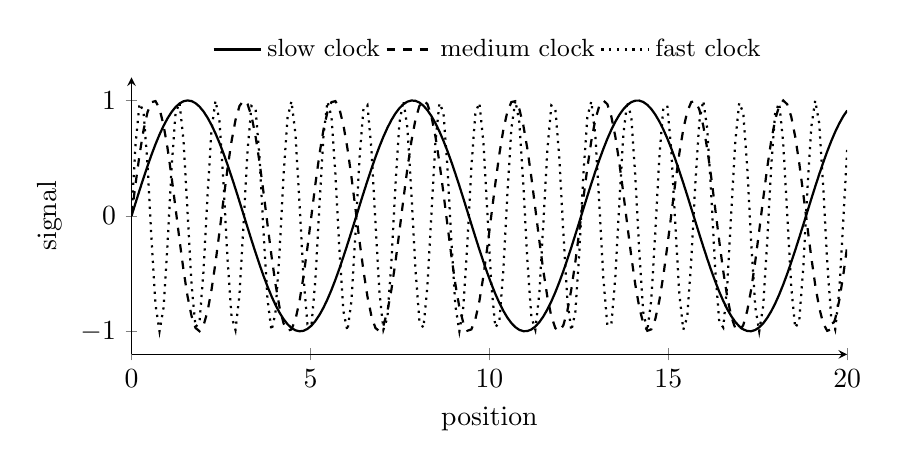
\begin{tikzpicture}
    \begin{axis}[
    width=.88\linewidth,height=5.1cm,
    axis lines=left,
    xlabel={position},
    ylabel={signal},
    xmin=0,xmax=20,ymin=-1.2,ymax=1.2,
    xtick={0,5,10,15,20},ytick={-1,0,1},
    legend style={draw=none,fill=none,font=\small,at={(.5,1.02)},anchor=south,legend columns=3}
    ]
    \addplot[domain=0:20,samples=180,thick] {sin(deg(x))};
    \addlegendentry{slow clock}
    \addplot[domain=0:20,samples=180,thick,dashed] {sin(deg(2.5*x))};
    \addlegendentry{medium clock}
    \addplot[domain=0:20,samples=180,thick,dotted] {sin(deg(6*x))};
    \addlegendentry{fast clock}
    \end{axis}
    \end{tikzpicture}
    \caption{Sinusoidal position uses many frequencies: a position is identified by the joint phase pattern rather than one scalar coordinate.}
    \label{fig:modern-sinusoidal-clocks}
\end{figure}
Position 17 produces one particular pattern across all those clocks.
Position 18 produces another.
Together, the frequencies form a distinctive coordinate system.
For those who are \textit{Physics minded} among you: this is analogous to using multiple Fourier frequencies.

\paragraph{Why the Trig?}
Because
\[
    \sin(a+b)=\sin a\cos b+\cos a\sin b,
\]
information about $\text{position}+k$ can be related algebraically to information about $\text{position}$.



\subsection{Relative Positional Embeddings}
\label{subsec:modern-relative-position}
The sinusoidal model is fundamentally given something resembling ``I am position 734''.
But many language relationships are naturally about ``that token is 3 tokens behind me'', which motivates \textbf{relative position}.
Consider:
\[
    \texttt{The dog that chased the cat was tired.}
\]
For many relationships, the important quantity is not
\[
    \texttt{dog}=\text{position }2,
    \qquad
    \texttt{cat}=\text{position }6,
\]
but something closer to
\[
    \texttt{cat is }+4\texttt{ relative to dog}.
\]

Relative positional methods inject information based on
\[
    \text{key position}-\text{query position}.
\]
Conceptually:
\[
    \underbrace{\text{token A}=500,\quad \text{token B}=503}_{\text{absolute}}
    \qquad\Longrightarrow\qquad
    \underbrace{\text{B is }+3\text{ from A}}_{\text{relative}}.
\]

\subsection{RoPE --- Rotary Positional Embeddings}
\label{subsec:modern-rope}
RoPE is one of the most important positional mechanisms.
Instead of adding a positional vector to the token embedding, RoPE \textit{rotates query and key vectors according to position}.
Take two dimensions of a query:
\[
    \begin{bmatrix}
    q_1\\q_2
    \end{bmatrix}.
\]
At position $m$, rotate them:
\[
    q'_m=R(m\theta)q \quad k'_n=R(n\theta)k,
\]
and calculate their dot product $(q'_m)^\top k'_n $:
\[
    q^\top R(m\theta)^\top R(n\theta)k 
    =
    R(m\theta)^\top R(n\theta)=R((n-m)\theta).
\]
So the interaction naturally depends on $n-m$:
\[
    (q'_m)^\top k'_n
    =
    q^\top R((n-m)\theta)k.
\]

\begin{figure}[htbp]
    \centering
    \begin{tikzpicture}[scale=1.05]
    \draw[->,draw=slate] (-.2,0)--(4.4,0) node[right,font=\small] {$q_1/k_1$};
    \draw[->,draw=slate] (0,-.2)--(0,3.8) node[above,font=\small] {$q_2/k_2$};
    \draw[arrblue] (0,0)--(3.2,.8) node[right,font=\small] {$R(m\theta)q$};
    \draw[arr] (0,0)--(1.7,2.7) node[above right,font=\small] {$R(n\theta)k$};
    \draw[draw=amber,thick] (1.0,.25) arc[start angle=14,end angle=58,radius=1.03];
    \node[font=\small,color=amber] at (1.5,.85) {$(n-m)\theta$};
    \node[yesbox] (rel) at (6.0,2.7) {Dot product depends on\\relative rotation};
    \draw[arr] (2.5,1.7)--(rel.west);
    \end{tikzpicture}
    \caption{RoPE turns position into phase: comparing two rotated vectors exposes their relative rotation.}
    \label{fig:modern-rope-geometry}
\end{figure}

\subsubsection*{Why RoPE is Elegant}
It contains both pieces of information:
\[
    \text{position }m\rightarrow\text{rotate }Q\text{ by }m\theta,
    \qquad
    \text{position }n\rightarrow\text{rotate }K\text{ by }n\theta.
\]
So absolute position is used to construct the representation, but \textbf{relative position emerges inside the attention interaction}.
This is a very attractive fit for attention.

\subsubsection*{Sinusoidal vs Relative vs RoPE}
\begin{center}
\small
\begin{tabularx}{.97\linewidth}{@{}L{.18\linewidth}L{.22\linewidth}YY@{}}
\toprule
\textbf{Method} & \textbf{Where position enters} & \textbf{Core idea} & \textbf{Inductive bias} \\
\midrule
Learned absolute & Token representation & Lookup position ID & Every position can learn its own identity \\
Sinusoidal & Token representation & Multiscale periodic coordinates & Smooth structured absolute position \\
Relative & Attention interaction & Explicitly encode displacement & Relationships depend on distance \\
RoPE & Rotate Q/K & Relative information emerges in dot product & Attention similarity should depend naturally on displacement \\
\bottomrule
\end{tabularx}
\end{center}

\begin{calloutmemoryhook}
Sinusoidal: give the token a coordinate.
Relative: tell attention the distance.
RoPE: rotate attention vectors so distance appears geometrically.
\end{calloutmemoryhook}

\subsection{YaRN}
\label{subsec:modern-yarn}
RoPE uses position to rotate queries and keys, but a model trained on a limited context has not learned to interpret arbitrarily large relative rotations.
\textbf{YaRN} (Yet another RoPE extensioN) extends the usable context of an existing RoPE model by changing the rotation frequencies and the scale of attention scores, usually followed by a small amount of long-context fine-tuning.

\paragraph{Interpolate, Rather Than Extrapolate}
A first attempt is \textbf{Position Interpolation}: compress positions so a longer sequence fits inside the original range.
For a model trained on $4\mathrm{k}$ tokens and extended to $64\mathrm{k}$, the position scale is $s=16$, so all RoPE rotations advance $16$ times more slowly.
This extends range but also reduces the angular difference between nearby tokens, weakening local position information.

\paragraph{NTK-by-Parts}
Recall that RoPE uses many rotation frequencies (like the sinusoidal bank of clocks in \cref{subsec:modern-sinusoidal-position}).
High-frequency dimensions rotate many times within the original context and provide fine positional detail; low-frequency dimensions rotate slowly and can help distinguish longer distances.
YaRN therefore \textbf{keeps short-wavelength rotations, stretches long-wavelength rotations, and blends those in-between}:
\[
    \underbrace{s}_{\text{context extension}}
    =\frac{N_{\text{target tokens}}}{N_{\text{trained tokens}}},
    \qquad
    \underbrace{\theta'_i}_{\text{new RoPE frequency}}
    =\underbrace{(1-\gamma_i)\frac{\theta_i}{s}}_{\text{extend long-range phase}}
    +\underbrace{\gamma_i\theta_i}_{\text{preserve local phase}}.
\]
The blending weight $\gamma_i$ runs from $0$ for long wavelengths to $1$ for short wavelengths.
This is called \textbf{NTK-by-parts interpolation}; unlike uniform interpolation, it does not sacrifice every positional frequency to gain context length.

\paragraph{Attention Temperature}
Extending the number of keys can make the attention distribution more diffuse.
YaRN also sharpens the attention logits before the softmax:
\[
    \underbrace{\operatorname{softmax}\!\left(
    \frac{Q_{\text{rotated}}K_{\text{rotated}}^\top}
    {\underbrace{t}_{\text{temperature}}\sqrt{N_{\text{key dims}}}}
    \right)}_{\text{attention over the extended context}},
    \qquad
    \underbrace{\frac{1}{\sqrt{t}}}_{\text{multiply both $Q$ and $K$ by this}}
    \approx 1+0.1\ln(s).
\]
The temperature rule is an empirical fit reported for LLaMA-family models, not a universal constant.
It can be folded into the RoPE query/key scaling, so it need not add a separate attention operation.

YaRN changes \textit{how positions are represented}, not how attention stores or searches history.
Long-context fine-tuning helps the model use the new positional range; it does not remove the extra attention and KV-cache cost of a longer sequence.
The original work extended Llama 2 models towards $64\mathrm{k}$ and $128\mathrm{k}$ contexts with comparatively little additional training.

% Source: Peng et al., YaRN: Efficient Context Window Extension of Large Language Models,
% ICLR 2024; https://arxiv.org/abs/2309.00071.